% ARPEGOS:  Automatized Roleplaying-game Profile Extensible Generator Ontology based System %
% Author : Alejandro Muñoz Del Álamo %
% Copyright 2019 %

% Section 11.1: Objetivos alcanzados %
\newpage
\section{Interfaz de usuario de \protege}
\textit{\textbf{Nota informativa}}: En este manual no se va a explicar cómo funcionan las ontologías, 
ni cómo funciona \protege, sino cómo desarrollar ontologías para juegos de rol específicas para este proyecto. \medskip

El primer paso para empezar a crear la nueva ontología de nuestro \textit{RPG} es abrir el editor.
Lo primero que se puede observar es una barra de direcciones, que normalmente aparece con el texto
\textit{untitled-ontology-x }, que es el nombre actual de la ontología, siendo x un número cualquiera. 
Esta barra además muestra el \textbf{IRI} (\textit{Internationalized Reference Identifier}) de la ontología. 
Esto es muy importante, pues todos los elementos de la ontología tienen 
su propio IRI, y cómo preámbulo utilizan el de la ontología a la que pertenecen. \medskip

\begin{figure}[H]
    \centering
    
\includegraphics[scale=0.8]{Figures/Protege/IRI_bar.png}
    \caption{Barra de dirección de \protege}
    \label{IRI_bar}
\end{figure}

A continuación aparece una barra de pestañas, cada una de las cuales hace referencia a una vista 
de \protege. \medskip
\begin{figure}[H]
    \centering
    
\includegraphics[scale=0.8]{Figures/Protege/Tab_bar.png}
    \caption{Barra de pestañas de \protege}
    \label{Tab_bar}
\end{figure}

De las pestañas que aparecen disponibles, sólo vamos a hacer uso de las tres primeras: \textit{Active Ontology}, 
\textit{Entities} e \textit{Individuals by class}, cada una de las cuales explicaremos en profundidad. Para más 
información, se recomienda consultar la documentación de \protege.

\newpage
\subsection{Active Ontology}
Esta vista permite configurar el IRI de ontología, el IRI de versión y las anotaciones de ontología de la 
ontología actual. Además, es posible asociar un prefijo al IRI de la ontología actual, e incluso importar otras 
ontologías existentes a la misma.\medskip

\begin{figure}[H]
    \centering
    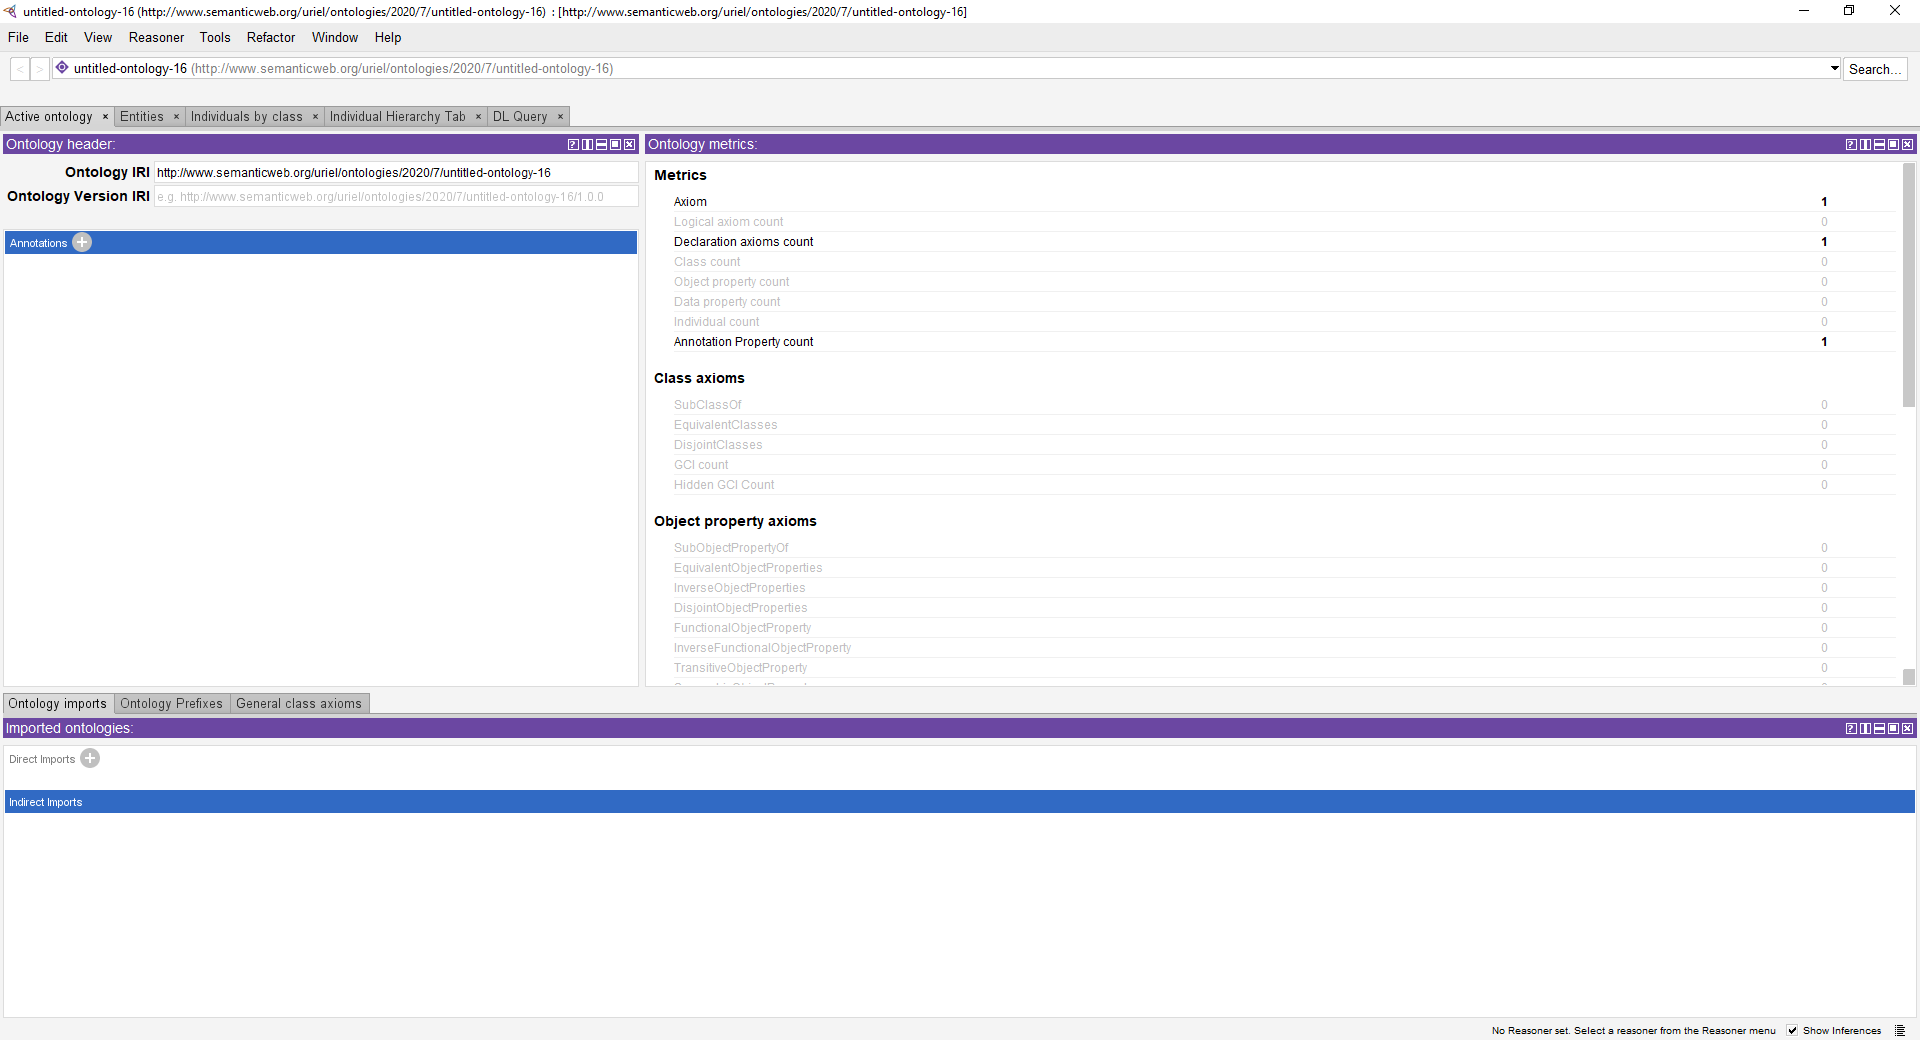
\includegraphics[scale=0.2]{Figures/Protege/Active_Ontology_view.png}
    \caption{Vista de la pestaña \textit{Active Ontology}}
    \label{Active_ontology_view}
\end{figure}

Comenzando por la zona superior izquierda está la vista \textit{Ontology Header}, la cual está formada 
por dos zonas claramente diferenciadas.\medskip

En la zona superior se pueden observar dos campos de texto, que permiten editar los IRIs de ontología y de versión
de ontología. Para el desarrollo de ontologías de este proyecto, se ha estimado conveniente utilizar un preámbulo genérico para 
la aplicación, el cual debe ser seguido por el nombre del juego. Así, por ejemplo, la ontología que ha desarrollado el equipo 
de desarrollo tiene el siguiente IRI: \medskip

\textit{\underline{urn:absolute:arpegos-project.org/games/}anima\_beyond\_fantasy}\medskip

En la zona inferior hay un campo en el que se pueden incluir anotaciones para la ontología. Se recomienda que todas las ontologías 
incluyan las siguientes anotaciones:

\begin{itemize}
    \item \underline{dc:title}: Anotación para indicar el título de la ontología
    \item \underline{dc:description}: Anotación para describir la ontología
    \item \underline{dc:creator}: Anotación para indicar el creador o los creadores de la ontología.
    \item \underline{dc:rights}: Anotación para indicar los derechos de la ontología.
\end{itemize}

La ontología de ejemplo muestra la vista \textit{Ontology Header} tal y como se muestra en la 
figura \ref*{Ontology_header}. \medskip

\begin{figure}[H]
    \centering
    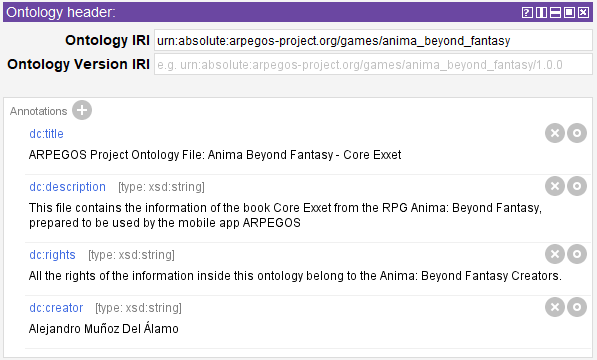
\includegraphics[scale=0.6]{Figures/Protege/Ontology_header.png}
    \caption{Anotaciones de la ontología}
    \label{Ontology_header}
\end{figure}

Al lado derecho de las anotaciones, están ubicadas las métricas de la ontología, que aportan toda la información 
referente a la ontología activa, como el número de axiomas existentes, separados según el tipo de axiomas y de elementos.
En el caso de la ontología elaborada por el equipo de desarrollo se han obtenido las métricas indicadas en la figura 
\ref*{Ontology_metrics}.

\begin{figure}[ht]
    \centering
    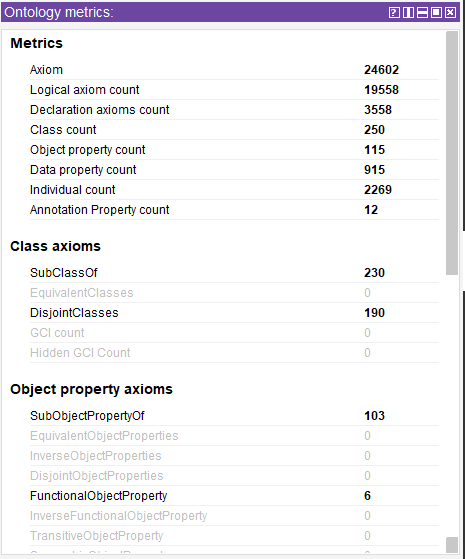
\includegraphics[scale=0.5]{Figures/Protege/Ontology_metrics.png}
    \caption{Métricas de la ontología}
    \label{Ontology_metrics}
\end{figure}

En la zona inferior de la pantalla, hay también otra barra de pestañas para trabajar con la ontología. 
De todas las disponibles sólo es necesaria aquella que tiene por nombre \textit{Ontology Prefixes}.
En esta vista se indican todos los prefijos disponibles en la ontología actual. Generalmente hay 
varios prefijos que aparecen siempre:

\begin{itemize}
    \item \textit{owl}: Hace referencia al estándar \textbf{OWL}.
    \item \textit{rdf}: Hace referencia al estándar \textbf{RDF}.
    \item \textit{rdfs}: Hace referencia al estándar \textbf{RDF Schema}.
    \item \textit{xml}: Hace referencia al estándar \textbf{XML}.
    \item \textit{xsd}: Hace referencia al estándar \textbf{XML Schema}.
\end{itemize}

Se recomienda asignar siempre un prefijo para la ontología que se desarrolle, de manera que se pueda acortar 
la referencia a cualquier elemento de la misma, usando el prefijo. En la figura \ref*{Ontology_prefixes} se 
muestran los prefijos disponibles para la ontología de \anima.\medskip

\begin{figure}[ht]
    \centering
    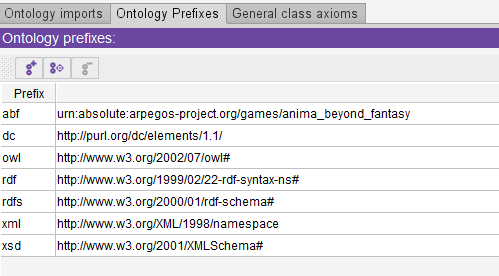
\includegraphics[scale=0.6]{Figures/Protege/Ontology_prefixes.png}
    \caption{Prefijos de la ontología}
    \label{Ontology_prefixes}
\end{figure}

\subsection{Entities}
Este apartado es uno de los más importantes de todo el programa, pues la mayoría del desarrollo se produce aquí.
Cuando se selecciona esta pestaña, aparece otra barra de pestañas justo debajo, como la que se puede apreciar 
en la figura \ref*{Entities_bar}. \medskip

\begin{figure}[H]
    \centering
    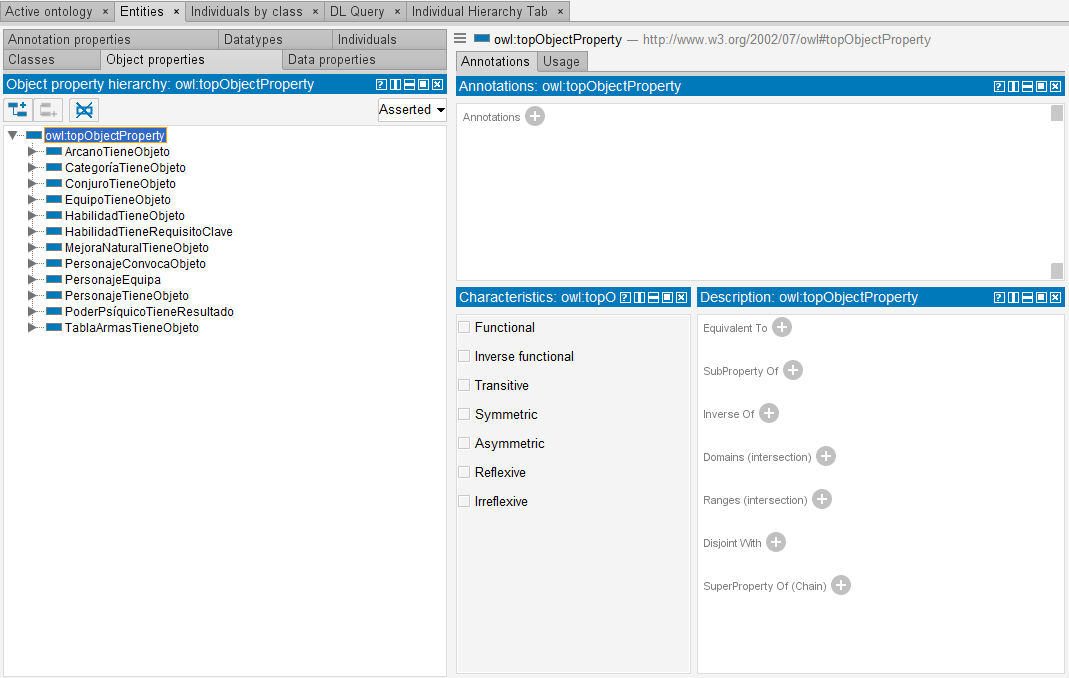
\includegraphics[scale=0.4]{Figures/Protege/Entities_workspace.png}
    \caption{Vista de la pestaña Entidades}
    \label{Entities_workspace}
\end{figure}

Aunque la barra dispone de seis opciones, las opciones estrictamente necesarias son las tres primeras 
opciones de izquierda a derecha:
\begin{itemize}
    \item \textit{Classes}: Esta opción muestra las clases de la ontología.
    \item \textit{Object Properties}: Aquí se muestran las propiedades de objeto. 
    \item \textit{Data Properties}: Esta opción muestra las propiedades de datos.
    \item \textit{Datatypes}: Esta opción muestra los diferentes tipos de valores de los que dispone la ontología.
\end{itemize}

\begin{figure}[H]
    \centering
    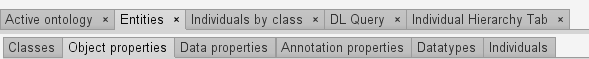
\includegraphics[scale=0.8]{Figures/Protege/Entities_bar.png}
    \caption{Barra de entidades}
    \label{Entities_bar}
\end{figure}


Asimismo, es posible distinguir dos espacios separados a izquierda y derecha. En el espacio izquierdo, se muestra 
la jerarquía de los elementos del tipo indicado en la barra de entidades, mientras que en el espacio derecho 
se muestran los detalles del elemento de la jerarquía seleccionado, mostrándose vacío mientras no haya ningún 
elemento seleccionado. La figura \ref*{Entities_workspace} ilustra lo previamente indicado. \medskip

El espacio derecho aparece generalmente separado en dos secciones: en la parte superior, una vista de las 
anotaciones del elemento seleccionado, y en la parte inferior, su descripción.\medskip

A continuación, se van a describir las diferentes vistas de descripción de cada una de las opciones disponibles en la barra de 
entidades.

\subsubsection{Classes}
En la figura \ref*{Class_details} aparecen las diferentes propiedades que puede tener una clase de una ontología, 
mostradas en la sección \textit{Description}:

\begin{figure}[H]
    \centering
    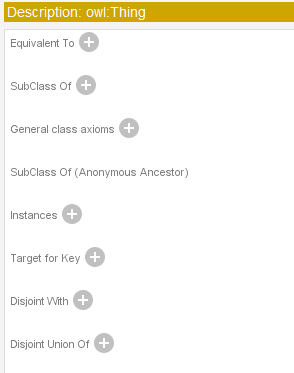
\includegraphics[scale=0.6]{Figures/Protege/Class_description.png}
    \caption{Vista de la sección \textit{Description} de la opción \textit{Classes}}
    \label{Class_details}
\end{figure}

\begin{itemize}
    \item \textit{Equivalent To}: Aquí se indican las clases que son equivalentes a la clase seleccionada.
    \item \textit{SubClass Of}: Aquí se muestran las clases a las que pertenece la clase seleccionada.
    \item \textit{General class axioms}: Este apartado expone los axiomas de clase generales en los que aparece la 
    clase seleccionada.
    \item \textit{Instances}: Los elementos aquí mostrados son los individuos que forman parte de la clase seleccionada.
    \item \textit{Target for Key}: Aqui se enseña una lista mixta de propiedades de objetos y datos que actuan como 
    claves para instancias de la clase seleccionada.
    \item \textit{Disjoint With}: Este apartado expone los elementos que son disjuntos con la clase seleccionada.
    \item \textit{Disjoint Union Of}: Aquí se muestran los axiomas de unión disjunta cuya clase principal es la clase seleccionada.
\end{itemize}

\subsubsection{Object Properties}
Las propiedades que aparecen en el apartado \textit{Description} de la opción 
\textit{Object Properties} varían un poco en comparación con las explicadas 
previamente, hecho que se puede apreciar en la figura \ref*{ObjectProperties_description}:

\begin{figure}[H]
    \centering
    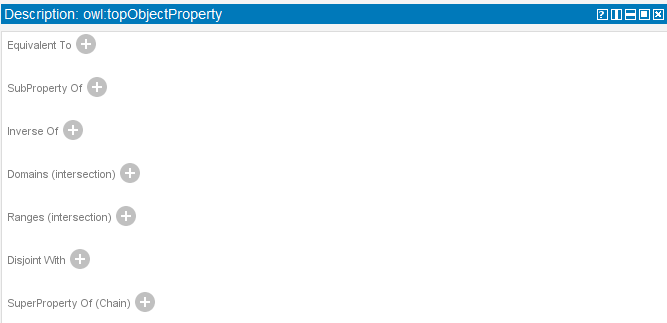
\includegraphics[scale=0.8]{Figures/Protege/ObjectProperties_description.png}
    \caption{Vista de la sección \textit{Description} de la opción \textit{Object Properties}}
    \label{ObjectProperties_description}
\end{figure}

\begin{itemize}
    \item \textit{Equivalent To}: Aquí se indican las propiedades equivalentes a la seleccionada.
    \item \textit{SubProperty Of}: Aquí se muestran las propiedades a las que pertenece la seleccionada.
    \item \textit{Inverse Of}: Este apartado expone las propiedades inversas a la seleccionada.
    \item \textit{Domains (intersection)}: Los elementos aquí mostrados son las clases o individuos que pueden 
    disponer de la propiedad seleccionada.
    \item \textit{Ranges (intersection)}: Aqui se enseñan las clases o individuos que pueden relacionarse con los elementos 
    del apartado \textit{Domains} mediante la propiedad seleccionada.
    \item \textit{Disjoint With}: Este apartado expone los elementos que son disjuntos con la clase seleccionada.
    \item \textit{SuperProperty Of (chain)}: La propiedad seleccionada es una superpropiedad de cada cadena de propiedades 
    mostradas en esta sección.
\end{itemize}

Además, la opción \textit{Object Properties} también dispone de una sección llamada \textit{Characteristics}, en la que 
se especifican algunas propiedades específicas de una propiedad de objeto (Figura \ref*{ObjectProperties_characteristics}). 

\begin{figure}[H]
    \centering
    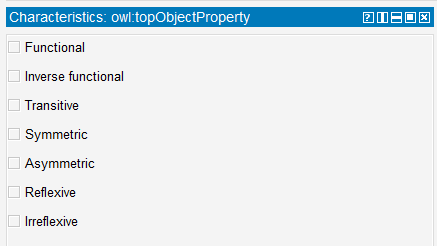
\includegraphics[scale=0.8]{Figures/Protege/ObjectProperties_characteristics.png}
    \caption{Vista de la sección \textit{Characteristics} de la opción \textit{Object Properties}}
    \label{ObjectProperties_characteristics}
\end{figure}

\begin{itemize}
    \item \textit{Functional}: A cada individuo del dominio (\textit{a}) sólo le corresponde un individuo del rango (\textit{b}).
    \item \textit{Inverse Functional}:  A cada individuo del rango (\textit{b}) sólo le corresponde un individuo del dominio (\textit{a}).
    \item \textit{Transitive}: Si un individuo \textit{a} esta relacionado con un individuo \textit{b}, y éste a su vez está
    relacionado con un individuo \textit{c}, entonces \textit{a} está relacionado con \textit{c}.
    \item \textit{Symmetric}: Si el individuo \textit{a} está relacionado con el individuo \textit{b}, entonces \textit{b} también 
    está relacionado con \textit{a} por medio de la misma propiedad.
    \item \textit{Asymmetric}: Si el individuo \textit{a} está relacionado con el individuo \textit{b}, entonces \textit{b} no 
    está relacionado con \textit{a} por medio de la misma propiedad.
    \item \textit{Reflexive}: Un individuo \textit{a} puede estar relacionado consigo mismo mediante la propiedad actual.
    \item \textit{Irreflexive}:Un individuo \textit{a} no puede estar relacionado consigo mismo mediante la propiedad actual.
\end{itemize}

\subsubsection{Data Properties}
Esta sección tiene la misma disposición que la opción \textit{Object Properties}, es decir, 
tiene un conjunto de propiedades en la vista \textit{Description}, mostradas en la figura 
\ref*{DataProperties_description}:

\begin{figure}[H]
    \centering
    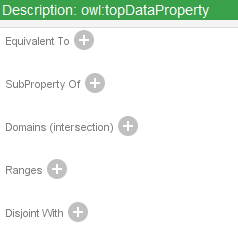
\includegraphics[scale=0.8]{Figures/Protege/DataProperties_description.png}
    \caption{Vista de la sección \textit{Description} de la opción \textit{Data Properties} }
    \label{DataProperties_description}
\end{figure}

\begin{itemize}
    \item \textit{Equivalent To}: Aquí se indican las propiedades equivalentes a la propiedad seleccionada.
    \item \textit{SubProperty Of}: Aquí se muestran las propiedades a las que pertenece la propiedad seleccionada.
    \item \textit{Domains (intersection)}: Los elementos aquí mostrados son las clases o individuos que pueden 
    disponer de la propiedad seleccionada.
    \item \textit{Ranges}: Aqui se enseñan las clases o individuos que pueden relacionarse con los elementos 
    del apartado \textit{Domains} mediante la propiedad seleccionada.
    \item \textit{Disjoint With}: Este apartado expone los elementos que son disjuntos con la clase seleccionada.
\end{itemize}

También dispone de un apartado \textit{Characteristics}, visible en la figura \ref*{DataProperties_characteristics}, 
aunque en este caso sólo hay opción disponible: \textit{Functional}, equivalente a la propiedad homónima del campo 
\textit{Object Properties}, salvando el hecho de que en vez de darse entre dos individuos, se da entre un individuo 
\textit{a} y un valor \textit{x}.

\begin{figure}[ht]
    \centering
    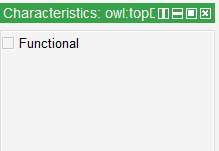
\includegraphics[scale=0.8]{Figures/Protege/DataProperties_characteristics.png}
    \caption{Vista de la sección \textit{Characteristics} de la opción \textit{Data Properties}}
    \label{DataProperties_characteristics}
\end{figure}

\subsubsection{Datatypes}
Los diferentes tipos de valores que puede tener cualquier propiedad de datos están declarados en este apartado (figura \ref*{Datatypes}).
Los más utilizados son los siguientes:
\begin{itemize}
    \item \textit{xsd:string}: Cadenas de caracteres y textos.
    \item \textit{xsd:integer}: Número enteros.
    \item \textit{xsd:unsignedInt}: Números enteros sin signo.
    \item \textit{xsd:float}: Números racionales.
    \item \textit{xsd:boolean}: Valores de verdadero o falso.
\end{itemize}


\begin{figure}[H]
    \centering
    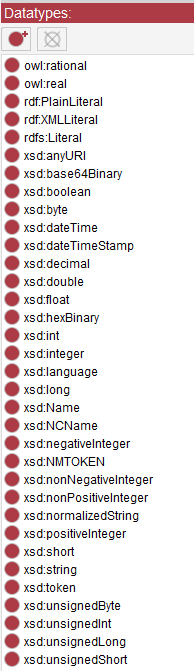
\includegraphics[scale=0.5]{Figures/Protege/Datatypes.png}
    \caption{Vista de la opción \textit{Datatypes}}
    \label{Datatypes}
\end{figure}


\subsection{Individuals by class}
Esta vista ofrece una vista global de la ontología, como se puede apreciar en la figura \ref*{IndividualsClass}. 
Esto se debe a que enseña diversos elementos que permiten conocer su estructura general, y muestra la 
información detallada de los elementos seleccionados.  

\begin{figure}[H]
    \centering
    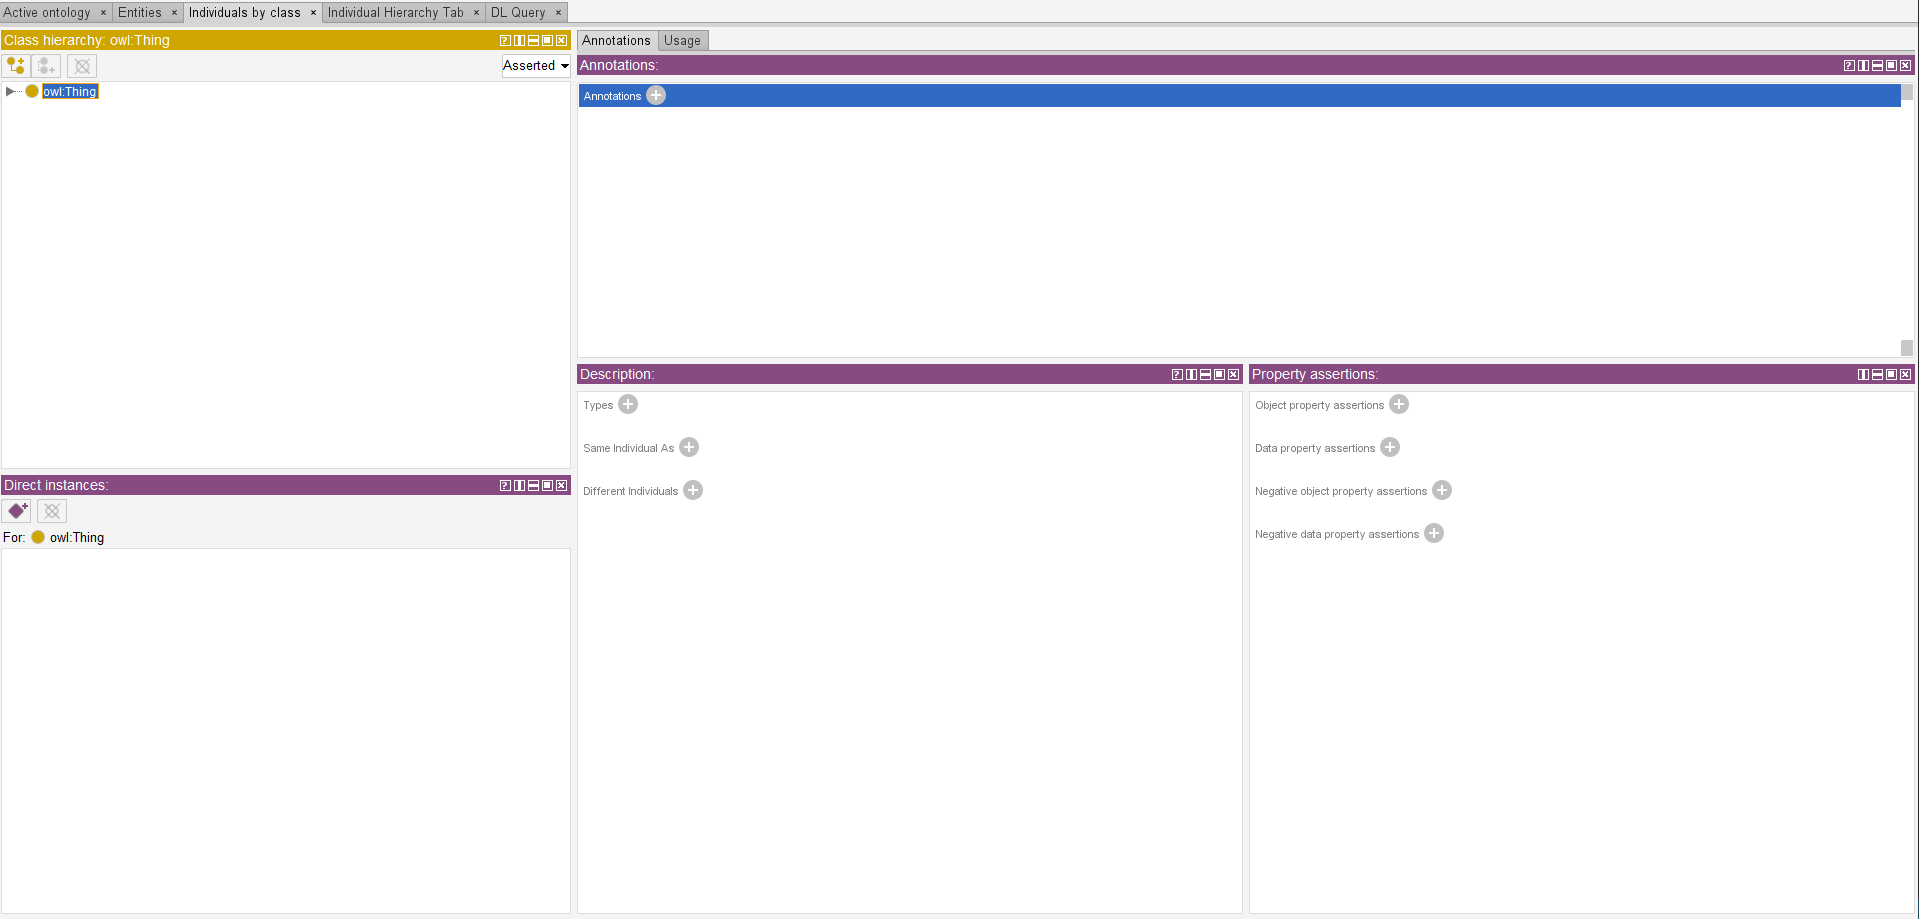
\includegraphics[scale=0.2]{Figures/Protege/IndividualsClass.png}
    \caption{Vista de la pestaña \textit{Individuals by Class}}
    \label{IndividualsClass}
\end{figure}

En la zona superior izquierda se encuentra la jerarquía de clases, de igual forma que en la opción \textit{Classes} de la 
pestaña \textit{Entities}. En la zona inmediatamente inferior, se puede apreciar una vista nueva, llamada \textit{Direct Instances}.
Esta vista muestra todos los individuos pertenecientes a la clase seleccionada en la jerarquía de clases. Esto se puede observar 
en la figura \ref*{IndividualsClass_Instances}.

\begin{figure}[H]
    \centering
    \includegraphics[scale=0.6]{Figures/Protege/IndividualsClass_Instances.png}
    \caption{Vista del apartado \textit{Direct Instances} de la pestaña \textit{Individuals by Class}}
    \label{IndividualsClass_Instances}
\end{figure}

Ubicado en la zona superior derecha, podemos ver el campo de anotaciones, que esta vez muestra aquellas relacionadas 
con el individuo seleccionado en el campo \textit{Direct Instances}. Una muestra de ello es la figura \ref*{IndividualClass_annotations}.

\begin{figure}[ht]
    \centering
    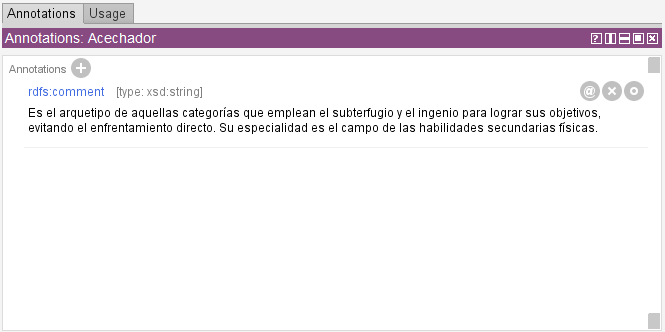
\includegraphics[scale=0.6]{Figures/Protege/IndividualsClass_annotations.png}
    \caption{Vista del apartado \textit{Annotations} de la pestaña \textit{Individuals by Class}}
    \label{IndividualClass_annotations}
\end{figure}

La zona inferior derecha está compartida entre dos vistas: 

\begin{itemize}
    \item \textit{Description}: Ubicada en la zona central de la pantalla (figura \ref*{IndividualClass_description}) muestra las características propias del 
    individuo seleccionado en el apartado \textit{Direct Instances}. Contempla tres tipos de características:
    \begin{itemize}
        \item \textit{Types}: Muestra todas las clases a las que pertenece el individuo seleccionado.
        \item \textit{Same Individual As}: Muestra los individuos equivalentes al seleccionado.
        \item \textit{Different Individuals}: Muestra los individuos establecidos como diferentes al seleccionado.
    \end{itemize}

    \item \textit{Property assertions}: Ubicada en la zona derecha (figura \ref*{IndividualClass_assertions}), permite observar 
    las propiedades de objeto y de dato directamente relacionadas con el individuo seleccionado como el que dispone de ellas. 
    Las propiedades que se muestran pueden ser de objeto y de dato, tanto afirmativas como negativas.

\end{itemize}


\begin{figure}[ht]
    \centering
    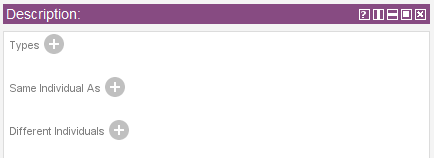
\includegraphics[scale=0.6]{Figures/Protege/IndividualsClass_description.png}
    \caption{Vista del apartado \textit{Description} de la pestaña \textit{Individuals by Class}}
    \label{IndividualClass_description}
\end{figure}


\begin{figure}[ht]
    \centering
    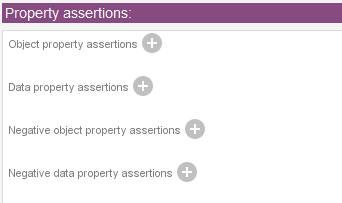
\includegraphics[scale=0.6]{Figures/Protege/IndividualsClass_assertions.png}
    \caption{Vista del apartado \textit{Description} de la pestaña \textit{Individuals by Class}}
    \label{IndividualClass_assertions}
\end{figure}